\documentclass[12pt,a4paper]{article}
\usepackage[utf8]{inputenc}
\usepackage[german]{babel}
\usepackage[T1]{fontenc}
\usepackage{amsmath}
\usepackage{amsfonts}
\usepackage{amssymb}
\usepackage{graphicx}
\usepackage[left=2.5cm,right=2.5cm,top=2cm,bottom=2cm]{geometry}
\author{Gruppe C14 \\ Julián Häck, Martin Koytek, Lars Wenning, Erik Zimmermann}
\usepackage{float}
\usepackage{multicol}
\begin{document}
\section{Kalibrierung des Temperatursensors}
Da wir bei der Hauptmessung einen Temperatursensor verwenden und nicht genau wissen, ob die angezeigte Temperatur am Cassy auch der tatsächlichen Temperatur entspricht, bestimmen wir in diesem Versuch den systematischen Fehler durch die Kalibrierung des Temperatursensors.

Beide Gruppen haben für die Kalibrierung des Temperatursensors  eine Rauschmessung mit Eiswasser in einem offenen Behälter durchgeführt. \newline
Bevor die tatsächliche Hauptmessung (Abkühlung) gemessen werden konnte, musste das Wasser zunächst auf Siedetemperatur erhitzt werden. Diese Temperatur ist sehr konstant und ist also gut geeignet, um ein Rauschen zu messen und damit die Temperatursensoren zu kalibrieren. \newline
Leider hat Gruppe 1 ihre Rauschmessung bei Siedetemperatur auf Geheiß eines Tutors verworfen \glqq for your eyes only\grqq.
Deshalb mussten wir hier allein auf die Messdaten von Gruppe 2 zurückgreifen.

\begin{figure}[hbtp]
\centering
\includegraphics[scale=0.5]{Bilder/Kalibration_Eiswasser.png}
\caption{Rauschmessung bei Eiswasser}
\end{figure}

\begin{table}[H]\centering
\caption{Rauschmessung der Temperatur beim Gefrierpunkt}
\begin{tabular}{c|c}
$T_M$ in K & 274.277  \\ 
$\sigma_T$ in K & 0.103  \\  
$\sigma_{T_M}$ in K & 0.002 \\  
$T_{Theo}$ & 272.2 \\
\end{tabular} 
\end{table}

\begin{figure}[H]
\centering
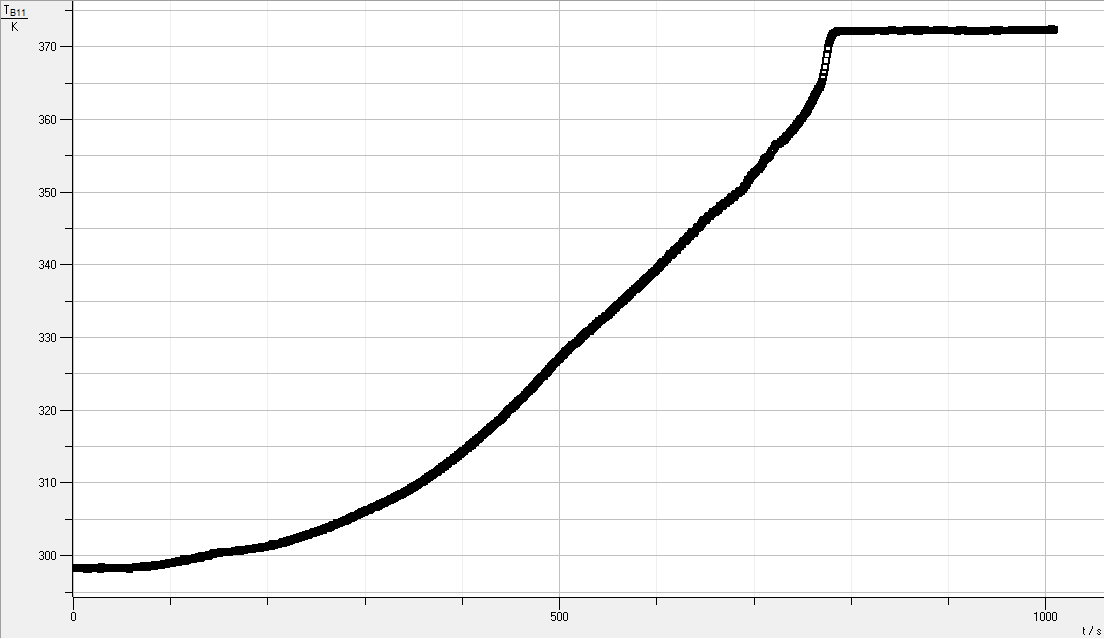
\includegraphics[scale=0.5]{Bilder/heizen.png}
\caption{Heizvorgang. Die Siedetemperatur ist erreicht, wenn die Kurve abflacht.}
\end{figure}

\begin{figure}[H]
\centering
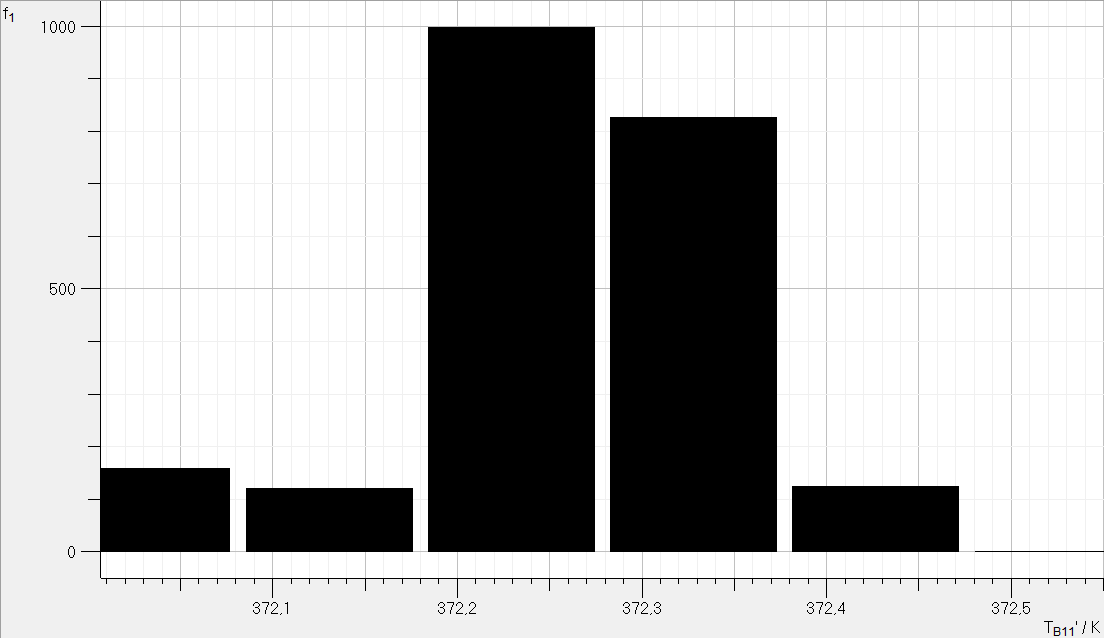
\includegraphics[scale=0.5]{Bilder/heizen_histogramm.png}
\caption{Kalibrierung bei Siedetemperatur.}
\end{figure}


\begin{table}[H]\centering
\caption{Rauschmessung der Temperatur beim Siedepunkt.}
\begin{tabular}{c|c}
$T_M$ in K & 372.227  \\
$\sigma_T$ in K & 0.083  \\
$\sigma_{T_M}$ in K & 0.002 \\
$T_{Theo}$ in K & 372.5 \\
\end{tabular} 
\end{table}
Der theoretische Wert für die Siedetemperatur ergibt sich aus dem Druck. Gemessen hat das Cassy bei Normalbedingungen im Labor einen Wert von: $p_C=1006.5$hPa. Die Wetterstation gab allerdings einen Wert von $p_W=984$hPa an. Also eine Differenz von $22.5$ hPa. Beim Sieden haben wir einen Druck von $1015 hPa$ gemessen. Mit der Korrektur von der Wetterstation ergibt sich also ein Druck von $p_{siede}=992.5hPa$. Bei diesem Druck ist eine Siedetemperatur von $99.4^{\circ}$ C zu erwarten, also 372.5K.  
\begin{figure}[H]
\centering
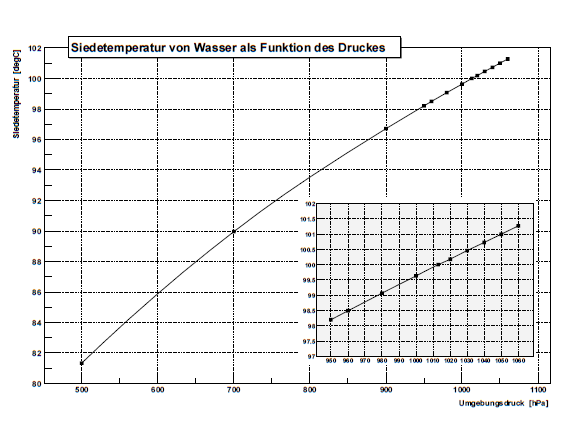
\includegraphics[scale=1]{Bilder/SiedeTemp_Druck.PNG}
\caption{Grafik aus dem Skript. Bei 992.5 hPa ist die Siedetemperatur 99.4 C.}
\end{figure}



Um nun von den von Cassy gemessenen Werte $T_C$ mit Fehlern $\sigma_{T_M}$ auf die realen Werte $T_R$ und ihre Fehler $\sigma_{T_{R}}$ zu kommen trägt man die theoretischen Werte gegen die gemessenen auf. Aus der Steigung und dem y-Achsen-Abschnitt ließe sich dann eine Umrechnung bestimmen.
\begin{equation}
T_{R}=aT_{C}+b
\end{equation}
Hätte man eine solche Formel könnte man durch Fehlerfortpflanzung den Fehler auf den realen  Messwert berechnen. 
\begin{equation}
\sigma_{T_{R}} = \sqrt{(T_C \sigma_a)^2+\sigma_b^2}
\end{equation}
Haben wir diesen Fehler können wir berechnen wie sich dieser dann auf die Werte der Hauptmessung niederschlägt und daraus die systematischen Fehler durch die Temperaturkalibrierung bestimmen. 
\begin{equation}
\sigma_{\lambda_{T}}=\frac{\sigma_T}{T}\cdot \Lambda
\end{equation}
Über eine Lineare Regression durch $T_{Schmelz}$ und $T_{Siede}$ mit ihren Fehlern legt kann man eine solche gesuchte Funktion finden. 
Damit die Werte beim Auftragen von $T_R$ gegen $T_C$ für Steigung und Y-Achsenabschnitt möglichst unkorreliert sind, verschieben wir die Y-Achse um den Mittelwert von Siedetemperatur und Schmelztemperatur.
\begin{equation}
\bar{T}=\frac{T_{Schmelz}+T_{siede}}{2}
\end{equation}
Die theoretischen Werte (y-Werte) sind also nicht fehlerbehaftet, $T_{Schmelz}$ und $T_{Siede}$ (x-Werte) allerdings schon. Leider haben wir in der Praktikumsbibliothek nur eine Funktion gefunden, die entweder Fehler auf beide Achsen akzeptiert oder nur Fehler auf y. \newline 
Deshalb haben wir die Gleichung invertiert und die so gefundene Steigung und Y-Achsenabschnitt in die eigentlich Gesuchten umgeformt.
Die eigentliche Gleichung wäre:
\begin{equation}
T_{R}=a_1(T_{C}-\bar{T})+b_1
\end{equation}
Die von uns zunächst bestimmte Gleichung ist:
\begin{equation}
(T_{C}-\bar{T})=a_2T_R+b_2
\end{equation}
\begin{figure}[H]
\centering
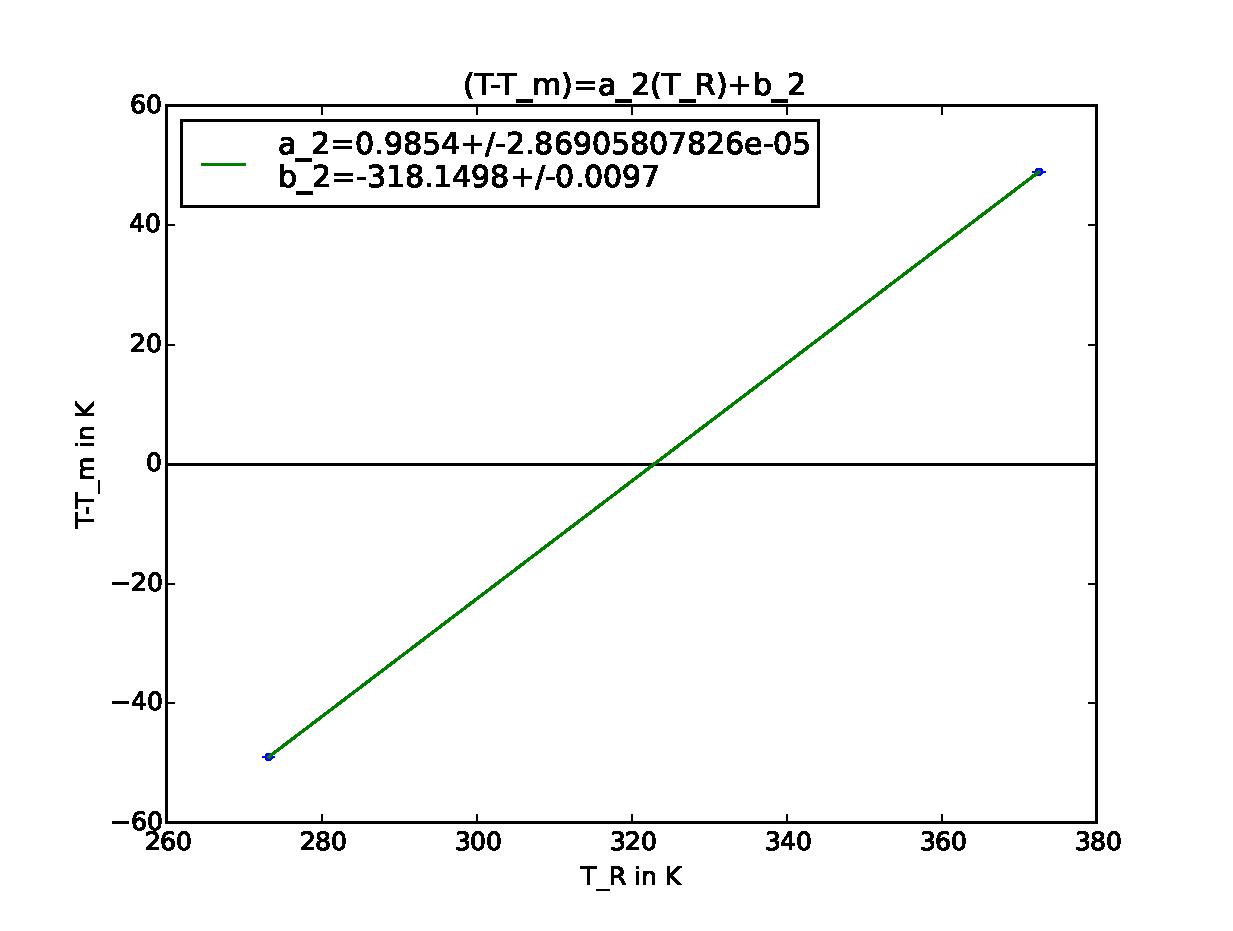
\includegraphics[scale=0.5]{Bilder/lineare_regression_T_kalibration.eps}
\caption{Lineare Regression zur Kalibrierung des Temperatursensors}
\end{figure}

\begin{equation}
a_2=0.985, \hspace{1cm} \sigma_{a_2}=2.870\cdot 10^{-5}\\
\end{equation}
\begin{equation}
b_2=-318.150 K, \hspace{1cm} \sigma_{b_2}=0.010 K
\end{equation}

Da die zweite Gleichung die invertierte der ersten ist, gilt, dass der X-Achsenabschnitt der einen dem Y-Achsenabschnitt der anderen Gleichung entspricht, und dass die eine Steigung die Inverse der anderen Steigung ist.
\begin{equation}
a_1=\frac{1}{a_2}, \hspace{1cm} \sigma_{a_1}=\frac{\sigma_{a_2}}{a_2^2}
\end{equation}
\begin{equation}
b_1=-\frac{b_2}{a_2}, \hspace{1cm} \sigma_{b_1}=b_1 \sqrt{(\frac{\sigma_{b_2}}{b_2})^2+(\frac{\sigma_{a_2}}{a_2})^2}
\end{equation}

Es gilt also:
\begin{equation}
a_1=1.015, \hspace{1cm} \sigma_{a_1}=2.955 \cdot 10^{-5}
\end{equation}
\begin{equation}
b_1=322.86 K, \hspace{1cm} \sigma_{b_1}=0.013 K
\end{equation}

\begin{figure}[H]
\centering
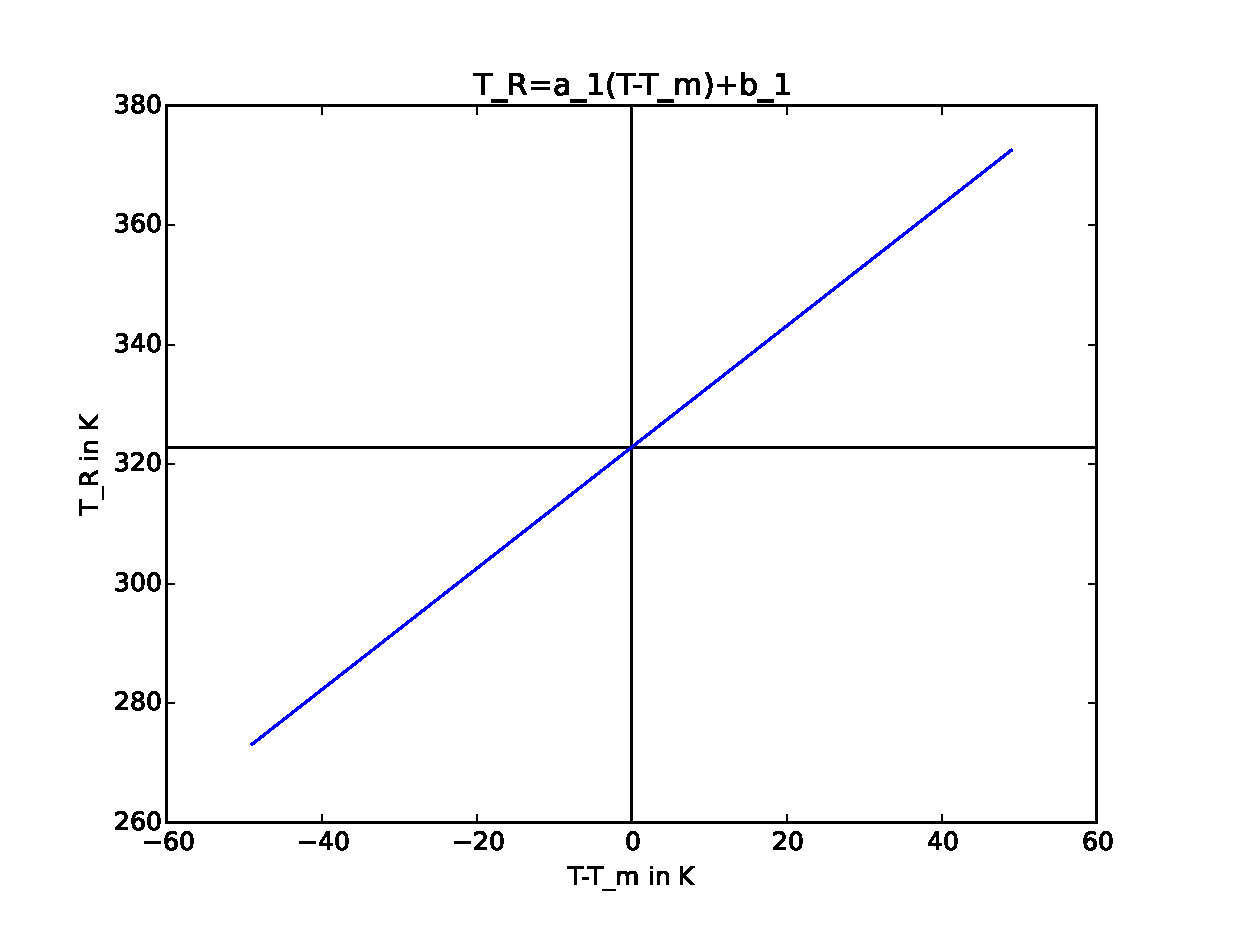
\includegraphics[scale=0.5]{Bilder/gewollteFunktion.eps}
\\
\caption{Funktion zur Kalibrierung}
\end{figure}


Wir haben nun alle Werte um den systematischen Fehler durch die Temperaturkalibrierung und damit den systematischen Fehler auf $\Lambda$ zu bestimmen.

\begin{equation}
\sigma_{T_{R}} = \sqrt{((T_C-\bar{T}) \sigma_a)^2+\sigma_b^2}=0.0137
\end{equation}

\begin{equation}
\sigma_{\lambda_{T}}=\frac{\sigma_T}{T}\cdot \Lambda= \sigma_{Kalibration}
\end{equation}

Aus den Herstellerangaben ergaben sich weitere systematische Fehler.

\begin{table}[H]\centering
\caption{Systematische Fehler aus Herstellerangaben: Druck}
\begin{tabular}{|c|c|}
\hline 
Linearitätsfehler & $\pm 1\%$ \\ 
\hline 
Sensor & $\pm 1\%$ \\ 
\hline 
Verstärkungsfehler & $\pm 1\%$ \\ 
\hline 
\end{tabular} 
\end{table}


\begin{table}[H]\centering
\caption{Systematische Fehler aus Herstellerangaben: Temperatur}
\begin{tabular}{|c|c|}
\hline 
Sensor & $\pm 2.5 K $ \\ 
\hline 
Konverter & $\pm 1\%$ \\ 
\hline 
\end{tabular}
\end{table}

Diese pflanzen sich wie folgt fort.
\begin{equation}
\sigma_{\Lambda,T} = \frac{\sigma_T}{T}\Lambda
\end{equation}
\begin{equation}
\sigma_{\Lambda,p} = RT\frac{\sigma_p}{p}
\end{equation}

\newpage
\begin{multicols}{2}
\begin{table}[H]\centering
\caption{Systematische Fehler Gruppe 1}
\begin{tabular}{c|c|c|c}
 &$\sigma_{Hersteller}$&$\sigma_{Kalibration}$&$\sigma_{Gesamt}$\\
\hline
$\Lambda_0$&0.513&0.002&0.513\\
$\Lambda_1$&0.519&0.002&0.519\\
$\Lambda_2$&0.534&0.002&0.534\\
$\Lambda_3$&0.515&0.002&0.515\\
$\Lambda_4$&0.526&0.002&0.526\\
$\Lambda_5$&0.537&0.002&0.537\\
$\Lambda_6$&0.532&0.002&0.532\\
$\Lambda_7$&0.53&0.002&0.53\\
$\Lambda_8$&0.513&0.002&0.513\\
$\Lambda_9$&0.547&0.002&0.547\\
$\Lambda_{10}$&0.517&0.002&0.517\\
$\Lambda_{11}$&0.514&0.002&0.514\\
$\Lambda_{12}$&0.535&0.002&0.535\\
$\Lambda_{13}$&0.563&0.002&0.563\\
$\Lambda_{14}$&0.499&0.002&0.499\\
$\Lambda_{15}$&0.506&0.002&0.506\\
$\Lambda_{16}$&0.521&0.002&0.521\\
$\Lambda_{17}$&0.488&0.002&0.488\\
$\Lambda_{18}$&0.528&0.002&0.528\\
$\Lambda_{19}$&0.458&0.001&0.458\\
$\Lambda_{20}$&0.468&0.001&0.468\\
\end{tabular}
\end{table}
\begin{table}[H]\centering
\caption{Systematische Fehler Gruppe 2}
\begin{tabular}{c|c|c|c}
 &$\sigma_{Hersteller}$&$\sigma_{Kalibration}$&$\sigma_{Gesamt}$\\
\hline
$\Lambda_0$&0.518&0.002&0.518\\
$\Lambda_1$&0.508&0.002&0.508\\
$\Lambda_2$&0.518&0.002&0.518\\
$\Lambda_3$&0.508&0.002&0.508\\
$\Lambda_4$&0.519&0.002&0.519\\
$\Lambda_5$&0.525&0.002&0.525\\
$\Lambda_6$&0.527&0.002&0.527\\
$\Lambda_7$&0.537&0.002&0.537\\
$\Lambda_8$&0.535&0.002&0.535\\
$\Lambda_9$&0.512&0.002&0.512\\
\end{tabular}
\end{table}
\end{multicols}

\section{Kalibrierung des Drucks}
Bei Zimmertemperatur haben beide Gruppen ihren Drucksensor kalibriert, indem der bei der Rauschmessung des Drucks gemessene Wert mit dem Wert der Wetterstation verglichen wurde.
\begin{table}[H]\centering
\begin{tabular}{|c|c|c|c|}
\hline 
 & $p_{Cassy}$ & $p_{Wetterstation}$ & $\Delta p$ \\ 
\hline 
Gruppe 1 & 981.54 hPa & 985 hPa & 3.46 hPa \\ 
\hline 
Gruppe 2 & 1006.5 hPa & 984 hPa & 22.5 hPa \\ 
\hline 
\end{tabular} 
\end{table}

Diese Abweichungen fallen bei der Hauptmessung allerdings nicht ins Gewicht, weil sie lediglich den Offset erhöhen würden aber nicht die Steigung verändern.

\end{document}